\documentclass[applsci,article,submit,pdftex,oneauthor]{Definitions/mdpi}

\usepackage{graphicx}
\usepackage{amsmath}
\usepackage{amssymb}
\usepackage{booktabs}
\usepackage{tabularx}

\firstpage{1}
\makeatletter
\setcounter{page}{\@firstpage}
\makeatother
\pubvolume{16}
\issuenum{1}
\articlenumber{0}
\pubyear{2026}
\copyrightyear{2026}
\datereceived{}
\daterevised{}
\dateaccepted{}
\datepublished{}
\hreflink{https://doi.org/}

\Title{Visual Partitions versus Per-Element Marking on Solid T-Beams}
\TitleCitation{Visual Partitions versus Per-Element Marking on Solid T-Beams}

\Author{Grok Build $^{1}$}
\AuthorNames{Grok Build}
\AuthorCitation{Grok Build}
\address{$^{1}$ \quad Computational mechanics campaign on CalculiX C3D8 T-beams.}
\corres{Correspondence: local computational record.}

\abstract{On a frozen-topology solid T-beam, every classical adaptive cycle pays for one global assembly and solve. Visual partitioning names a few structural regions, writes a size on each, and rebuilds a conforming mesh three times. This paper compares those two discretisation philosophies on the same object: a three-dimensional C3D8 cantilever in CalculiX~2.23. The classical side is per-element Zienkiewicz--Zhu / residual D{\"o}rfler marking ($\theta=1/2$) with hanging 8-splits, and per-element Houston--Wihler local $hp$ prediction ($\theta=1/3$), which is not a partition. The visual side is a log-linear size field through named regions (clamp face, flange--web re-entrant corner, tip flange, plus a distinctive feature on each taper), one residual revision, and a one-generation two-coordinate particle swarm. Error is measured against a uniform $h=20\,\mathrm{mm}$ C3D8 reference, not against Euler--Bernoulli theory. On prismatic G01 under linear static load, three partition solves give $e_u=3.58\%$, $2.90\%$, $2.91\%$ at $N=5184$, $6048$, $6048$ equations. Per-element ZZ--D{\"o}rfler at the same three global solves remains at $16.1\%$, $15.5\%$, $13.7\%$. The D{\"o}rfler curve is continued to eight points until an equation cap; it is not a three-point method and it is not a partition. A six-zone spanwise template is not a method of this paper.}

\keyword{adaptive mesh refinement; T-beam; visual partition; size field; D{\"o}rfler marking; Houston--Wihler; CalculiX}

\begin{document}

\section{Introduction}
\label{sec:intro}

A solid T-beam is not a model elliptic equation on a uniform grid. The clamp face, the flange--web re-entrant corner, and the free-end load introduction each ask for local resolution. Uniform hexahedra spend most of their degrees of freedom in the smooth mid-span. Adaptive mesh refinement answers that request by a loop: solve, estimate, mark, refine~\citep{ZienkiewiczZhu1987,Doerfler1996,Chamoin2021}. D{\"o}rfler's object is the element $K$~\citep{Doerfler1996}. Houston and Wihler's object is the face-neighbour patch of each hex $\kappa$~\citep{HoustonWihler2016}. Neither paper partitions the domain into named structural blocks.

Engineers often do the opposite. They look at the structure, name a few parts, and write a size on each part. The mesh is then generated from a size field. That is a partition. A short loop---vision sizes, one residual revision, two-coordinate calibration---uses three global solves. The scientific question is where that short loop sits relative to a per-element marking loop, read at matched equation counts \emph{and} at matched numbers of global solves.

This paper reports one CalculiX campaign on that question. It does not treat D{\"o}rfler as a partition, it does not treat Houston--Wihler as a partition, and it does not revive a six-zone spanwise template that exists in the repository as a 2026-08-15 coding artefact. The contribution is a comparison of two discretisation philosophies on one solid T-beam family, not a new graph network.

\section{Related Work}
\label{sec:rw}

\subsection{Per-element $h$-adaptivity}

D{\"o}rfler proved that bulk marking by a collective fraction $\theta$ of $\sum\eta_K^2$, followed by refinement and re-solve, converges for Poisson~\citep{Doerfler1996}. The marked object is the element. Morin, Nochetto and Siebert identified data oscillation~\citep{Morin2000}; Casc{\'o}n et al.\ obtained quasi-optimal rates~\citep{Cascon2008}. None of those theorems define the tip displacement after two cycles as the truth. This paper takes the 1996 element object, $\theta=1/2$, and hanging 8-split as the classical $h$ protocol. Simple nodal-averaging Zienkiewicz--Zhu recovery~\citep{ZienkiewiczZhu1987} is the working indicator (not superconvergent patch recovery). Residual indicators on C3D8 one-point stresses are run as a separate loop. Amor-Mart\'in and Garcia-Castillo discuss conforming steps that avoid hanging nodes in prismatic electromagnetics~\citep{AmorMartin2021}; that literature is not a licence to rewrite D{\"o}rfler's object as a spanwise station cut.

\subsection{Local energy prediction is not a partition}

Houston and Wihler pose a pair of local Dirichlet problems on $T_\kappa^N=\{\kappa\}\cup$ face neighbours, compare predicted drops in potential $E_D=\tfrac12 a(u,u)-\ell(u)$, and mark by the maximal rule~\eqref{eq:hwmark} with $\theta=1/3$~\citep{HoustonWihler2016}. Algorithm~1 line~14 returns to the global solve. Example~1 of that paper reports an $hp$ mesh after nine adaptive refinements. The patch travels with $\kappa$; it is not a partition of $\Omega$. Babu{\v{s}}ka and Rheinboldt used vertex-star Dirichlet problems~\citep{BabuskaRheinboldt1978}. Bammer, Schr{\"o}der and Wihler later wrote an abstract loop~\citep{Bammer2025}. This paper keeps Houston--Wihler marking at (4.12) and does not mix D{\"o}rfler into that outer loop. On a three-dimensional face-neighbour patch, quadratic serendipity hexes have every node on $\partial D(\kappa)$, so the $p$-problem is empty. The $p$-branch here is an in-process 27-node $Q2$ assembly; CalculiX~2.23 is never sent \texttt{TYPE=C3D27}.

\begin{equation}
\Delta\widetilde E_{\kappa,\max}>\theta\max_{\kappa'}\Delta\widetilde E_{\kappa',\max},\qquad\theta=\tfrac13.
\label{eq:hwmark}
\end{equation}

\subsection{Size fields and learning}

MeshingNet, LAMG and AMBER predict a size field and often retain only a global scalar to meet a budget. Loseille--Alauzet continuous mesh theory treats an embedded family as a global scaling of a fixed anisotropic shape. The two-coordinate particle swarm in this paper is that remaining freedom after a regional step, not the partition itself. Yang, Foucart, and ASMR write \emph{marking} as a Markov decision process with the element as the agent~\citep{Yang2023,Foucart2023}. Those works are learned per-element markers, not partitions. They are discussed, not retrained, here.

\section{Materials and Methods}
\label{sec:mm}

\subsection{Geometry, material, load cases}

Units are mm, N, MPa, t, s. The solver is CalculiX~2.23 with SPOOLES, entry \texttt{/workspace/agentic-work/ccx}, binary SHA-256 \texttt{31be21fc2f0902bd9a05acc2651dbac6dc2a2573dabbf235e39a38cb6f458862}. Global elements are C3D8. Through-T counts are frozen at web $2\times 5$, outrigger $4$, flange thickness $2$, passed explicitly so automatic through-counts cannot add layers.

Prismatic G01 is the extrusion of flange $240\times 20$ and web $20\times 140$ over $L=2000\,\mathrm{mm}$, volume $1.52\times 10^7\,\mathrm{mm}^3$, from \texttt{tbeam\_solid\_hex.py}. T01--T10 are the ten families in \texttt{tbeam\_taper.py}. T01 is a linear haunch (web height $200\to 80\,\mathrm{mm}$ with a level top at $z=220$), not an alias of G01. The coarse identity T0 is \texttt{uniform\_x\_stations(18)}: 18 spanwise cells, 540 hexes, 912 nodes, 2592 unconstrained equations, verified on all eleven beams.

Steel is illustrative: $E=2.1\times 10^5\,\mathrm{MPa}$, $\nu=0.3$, $\rho=7.85\times 10^{-9}\,\mathrm{t\,mm}^{-3}$, $f_y=235\,\mathrm{MPa}$. Five load cases: S-LIN ($-5000\,\mathrm{N}$ on the tip-top set), S-ISO and S-KIN (plastic resultant from the root-section fibre formula with factor $1.35$), D-LIN ($-8000\,\mathrm{N}$) and D-NLG ($-30000\,\mathrm{N}$) with the same pulse. S-KIN's second step is $-0.5F$, not a full reversal. Houston--Wihler is run only on S-LIN.

The S-LIN error is
\begin{equation}
e_u=\frac{|u_z-u_z^{\mathrm{ref}}|}{|u_z^{\mathrm{ref}}|},\qquad
u_z=\mathrm{mean}\{U_3(n):n\in\mathrm{TIP\_TOP}\},
\end{equation}
with $u_z^{\mathrm{ref}}$ from a uniform $h=20\,\mathrm{mm}$ C3D8 mesh on the same section law (100 spanwise cells). Euler--Bernoulli tip displacement is tabulated as an order-of-magnitude column and is not an error axis.

\subsection{Visual partition}

G01 S-LIN uses three named regions: clamp face ($x_i=40\,\mathrm{mm}$, $h=42$), flange--web junction ($120$, $50$), tip-flange load ($1960$, $64$). Other load cases add a fourth structural region. Each taper adds one distinctive feature. Region count follows the view; it is not six. The size field is log-linear in $x$ between ordered anchors $(x_i,h_i)$, constant outside the first and last anchor. Spanwise stations are generated by \texttt{tbeam\_taper.build\_x\_stations} applied to that field. Vision box mid-points are not used as station generators.

After the delegated solve, residual $\eta_{K,R}^2$ is summed in spanwise Voronoi cells of the anchors. One call of \texttt{algorithm\_from\_mapping.run} with the default \texttt{AlgorithmConfig} ($pso\_generations=1$, seed 17) produces a mother-particle size vector and a selected-particle vector. Each is remeshed from scratch and solved. The three equation counts are required to be distinct; collisions are recorded and not plotted as fake iterations. D{\"o}rfler is not cancelled when the third partition point collides.

\subsection{Per-element D{\"o}rfler}

Indicators are $\eta_{K,\mathrm{ZZ}}^2$ from simple recovery and $\eta_{K,R}^2$ from face jumps, computed per hex id. Marking is \texttt{doerfler\_mark} with $\theta=1/2$. Refinement is \texttt{refine\_marked\_hexes} with 1-irregular closure and CalculiX \texttt{*EQUATION}. Spanwise station bisection is not used. The loop stops at the first of: empty mark set; $N\ge N_{\mathrm{cap}}$; twelve refinements. $N_{\mathrm{cap}}=\min(4N_{\mathrm{PSO}},N_{\mathrm{ref}})$ when a distinct third partition point exists, otherwise $N_{\mathrm{ref}}$. Relative drops in $e_u$ are diagnostic, not a stop. G01 ZZ is required to produce at least eight points unless the mark set empties or $N_{\mathrm{ref}}$ is hit.

\subsection{Houston--Wihler}

Local $h$ is an 8-split of $T_\kappa^N$. Local $p$ is in-process $Q2$. After the first hanging 8-split, $T_\kappa^N$ uses matching-face adjacency plus the undirected hanging-face neighbourhood from the coarser-neighbour geometry test. Hanging slave nodes are removed from the local free set. Global mixed-order meshes are not hung: every marked hex, including $p$-winners, is 8-split globally, and $n_{p\text{-realized-as-}h}=|p\text{-marked}|$ is recorded. R8 checks four conformal seeds (clamp web, re-entrant, mid-span, tip flange) plus one hanging-interface seed.

\section{Results}
\label{sec:results}

All numbers below come from \texttt{artifacts/amr\_plan\_run/} of this run. Old manuscript percentages are not reused.

\subsection{References and T0}

On G01 S-LIN the $h=20\,\mathrm{mm}$ reference has $N=14400$ equations and $u_z^{\mathrm{ref}}=-3.9674\,\mathrm{mm}$. T0 has $N=2592$, $u_z=-3.3288\,\mathrm{mm}$, $e_u=16.10\%$. The same T0 counts (540/912/2592) hold on T01--T10. A G01 $h=28\,\mathrm{mm}$ C3D8 card has $N=10368$. A C3D20 card on the T0 layout has $N=9573$ and completed. Reaction force on the clamp closes to the applied load at relative level $10^{-3}$ or better on the linear static cards.

T01 is not G01: its reference tip displacement is $-2.7185\,\mathrm{mm}$ against G01's $-3.9674\,\mathrm{mm}$.

\subsection{Visual partition, S-LIN}

Table~\ref{tab:llm} lists the three partition solves. On G01 the delegated, revision and PSO meshes have $N=5184$, $6048$, $6048$. The last two collide; that collision is recorded and the two points are not drawn as a fake third iterate. $e_u$ is $3.58\%$, $2.90\%$, $2.91\%$. Six of the ten tapers produce three distinct $N$.

\begin{table}[H]
\caption{S-LIN visual-partition short loop. $e_u$ relative to the $h=20\,\mathrm{mm}$ C3D8 reference. Distinct $N$ is a gate, not a smoothness claim.}
\label{tab:llm}
\begin{tabular}{lrrrccc}
\toprule
Beam & $N_{\mathrm{del}}$ & $N_{\mathrm{rev}}$ & $N_{\mathrm{pso}}$ & distinct & $e_u$ del/rev/pso & $(s,\kappa)$ \\
\midrule
G01 & 5184 & 6048 & 6048 & no & 3.58 / 2.90 / 2.91 & $(0.00,0.04)$ \\
T01 & 5184 & 5328 & 5328 & no & 3.53 / 3.63 / 3.69 & $(0.00,0.04)$ \\
T02 & 5184 & 5760 & 5904 & yes & 5.11 / 3.98 / 3.66 & $(-0.039,0)$ \\
T03 & 5040 & 5328 & 5328 & no & 6.96 / 5.38 / 5.38 & $(0.00,-0.04)$ \\
T08 & 5184 & 5328 & 5328 & no & 3.48 / 3.33 / 3.36 & $(0.00,0.04)$ \\
T09 & 5184 & 5904 & 5760 & yes & 8.33 / 5.87 / 6.01 & $(0.039,0)$ \\
\bottomrule
\end{tabular}
\end{table}

\subsection{Per-element hanging D{\"o}rfler}

G01 ZZ--D{\"o}rfler ran eight cycles (T0 through cycle~7) and stopped on the equation cap (Table~\ref{tab:zz}). Marked-hex counts are 33, 132, 130, 165, 212, 297, 395, 1172. $e_u$ falls from $16.1\%$ to $6.11\%$. It does not jump to a few percent in two cycles. T01 and T08 were run to the same stop (eight and six points). T02--T07, T09, T10 are T0 plus two cycles (existence), labelled as such in Figure~\ref{fig:ten}. G01 residual D{\"o}rfler (hanging-face jumps not area-weighted; the stop was not changed) has six points, last $e_u=7.76\%$ at $N=20265$. A single uniform 8-split of every T0 hex produces 4320 hexes, $N=16740$, $e_u=4.10\%$.

\begin{table}[H]
\caption{G01 S-LIN hanging ZZ--D{\"o}rfler. Encryption atom: 8-split of marked hexes plus 1-irregular \texttt{*EQUATION}. Not station bisection.}
\label{tab:zz}
\begin{tabular}{crrrr}
\toprule
cycle & $N$ & $n_{\mathrm{hex}}$ & $n_{\mathrm{marked}}$ & $e_u$ \\
\midrule
0 & 2592 & 540 & 33 & 0.1610 \\
1 & 3216 & 771 & 132 & 0.1553 \\
2 & 4371 & 1184 & 130 & 0.1373 \\
3 & 5484 & 1618 & 165 & 0.1232 \\
4 & 6999 & 2227 & 212 & 0.1143 \\
5 & 8970 & 3018 & 297 & 0.1028 \\
6 & 12174 & 4250 & 395 & 0.0833 \\
7 & 16911 & 6077 & 1172 & 0.0611 \\
\bottomrule
\end{tabular}
\end{table}

\subsection{Matched solves and matched $N$}

Figure~\ref{fig:solves} is the comparison the question asks for. The partition abscissa is 1, 2, 3. D{\"o}rfler is counted from cycle~0. At three global solves, G01 partition $e_u$ is $2.9\%$; ZZ--D{\"o}rfler is $13.7\%$. Figure~\ref{fig:n} uses $n_{\mathrm{equations}}$. At $N\approx 5500$--$6000$, partition $e_u\approx 2.9\%$ while ZZ at $N=5484$ is $12.3\%$. The two meshes do not share an atom: the caption of each figure states that the partition mesh is a conforming size field and the D{\"o}rfler mesh is hanging 8-split. A uniform conforming ladder on G01 gives $e_u=16.1\%$, $5.48\%$, $2.21\%$ at $N=2592$, $4608$, $6912$.

\begin{figure}[H]
\centering
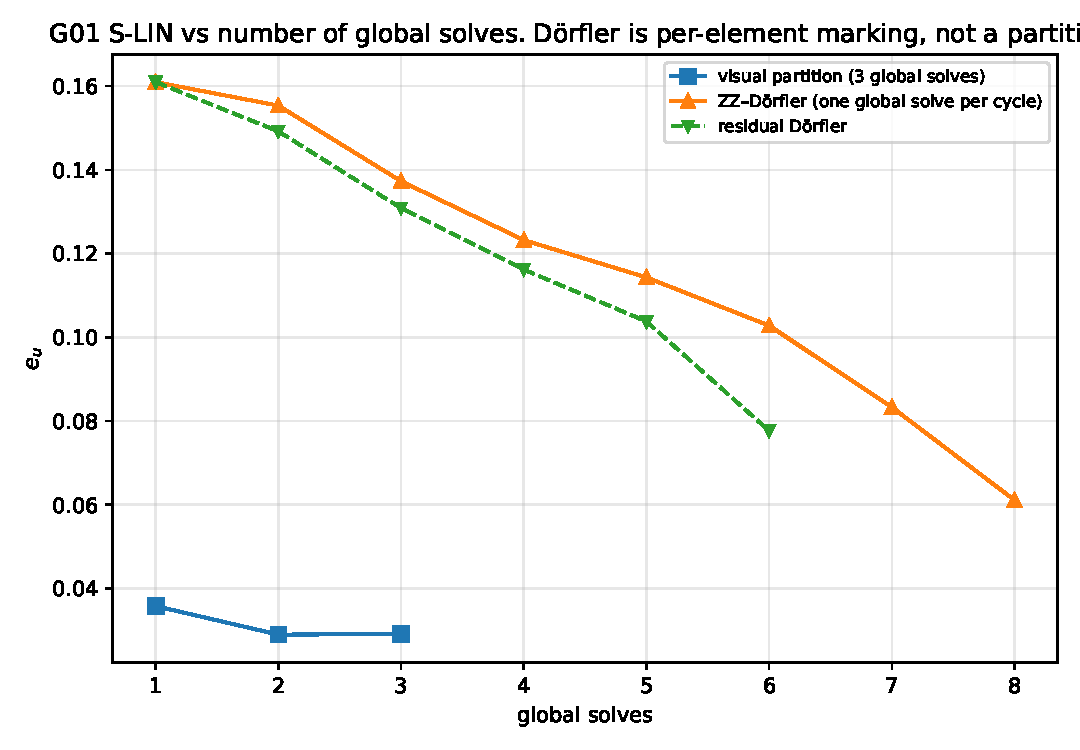
\includegraphics[width=0.85\textwidth]{figures/fig05_g01_eu_vs_solves.pdf}
\caption{G01 S-LIN, $e_u$ against the number of global solves. Blue squares: visual partition. Orange triangles: per-element ZZ--D{\"o}rfler (hanging 8-split). D{\"o}rfler is not a partition.}
\label{fig:solves}
\end{figure}

\begin{figure}[H]
\centering
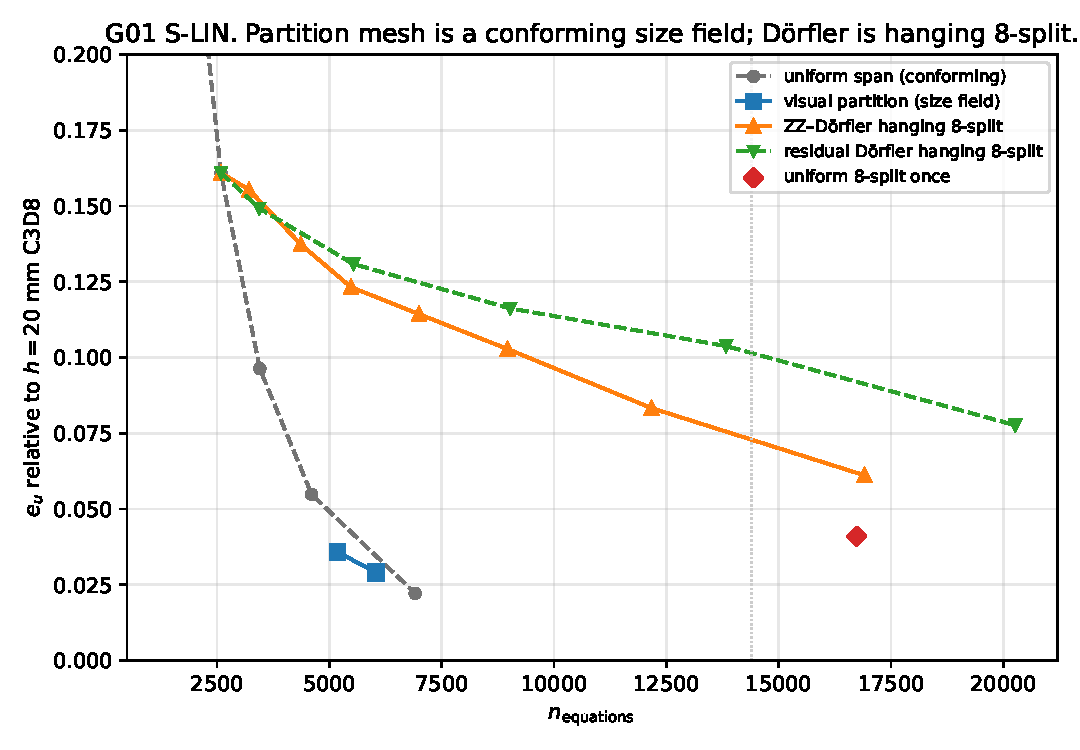
\includegraphics[width=0.85\textwidth]{figures/fig04_g01_eu_vs_N.pdf}
\caption{G01 S-LIN, $e_u$ against $n_{\mathrm{equations}}$. Partition points are a conforming size field; D{\"o}rfler points are hanging 8-split. Uniform spanwise ladders and one uniform 8-split are not marking methods.}
\label{fig:n}
\end{figure}

\begin{figure}[H]
\centering
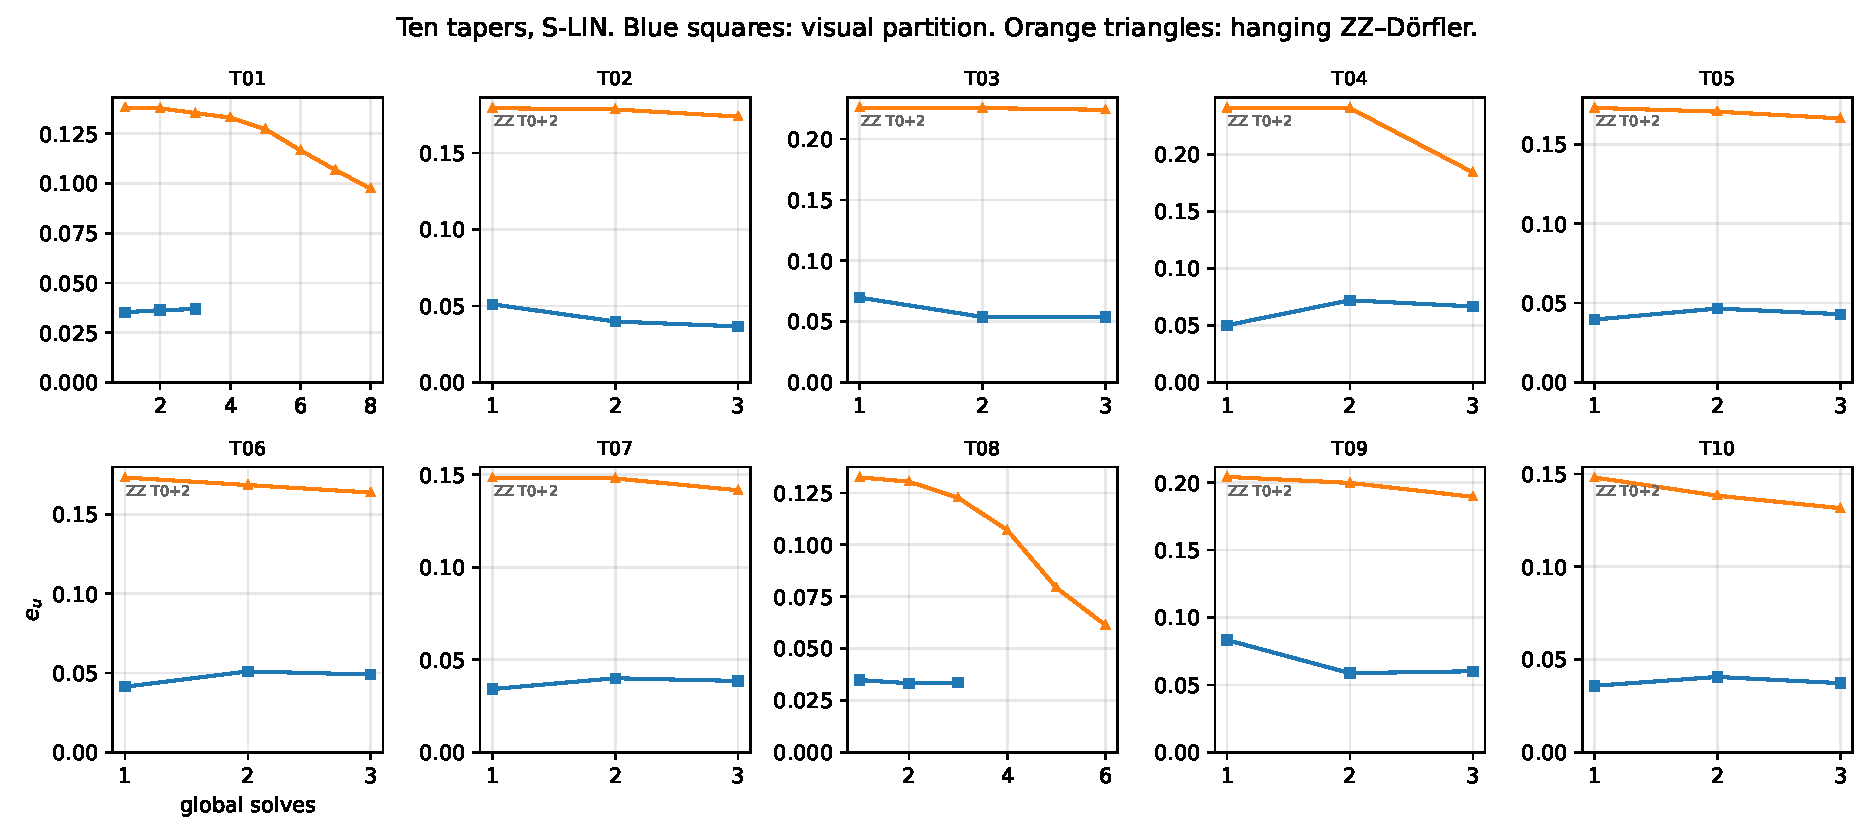
\includegraphics[width=0.98\textwidth]{figures/fig08_ten_family_solves.pdf}
\caption{Ten tapers, S-LIN, global-solve axis. Blue: visual partition (three solves). Orange: hanging ZZ--D{\"o}rfler. Panels with only T0$+$2 D{\"o}rfler points are existence runs, not full curves.}
\label{fig:ten}
\end{figure}

\subsection{Local prediction (R8), not a partition}

On G01 T0 the four conformal seeds are eid 2 (clamp web), 49 (re-entrant), 243 (mid-span), 532 (tip flange). In-process $Q2$ has $n_{\mathrm{free}}=9,13,11,9>0$ and finite $\Delta E_p$. Unenriched in-process C3D8 ALLSE matches the assembler. In-process $h$ ALLSE matches a CalculiX 8-split local job to relative error $<10^{-4}$ on the first three seeds. The tip seed's potential comparison is dominated by the load term on Dirichlet nodes; ALLSE on that seed still drops. After one 8-split of the re-entrant hex, a fine hex (eid 19) has four hanging-face neighbours. In-process $\Delta E_h$ and $\Delta E_p$ on that hanging patch are finite. The Houston--Wihler outer loop to nine cycles is not completed in this artefact set; R8 is the gate that was run. Local prediction is not drawn as a partition in any figure.

\subsection{Nonlinear cards}

The twelve required nonlinear cells (G01, T01, T08 $\times$ S-ISO, S-KIN, D-LIN, D-NLG) all produced three CalculiX jobs. Distinct $N$ holds on G01 S-ISO ($5040,5616,5904$), T01 S-ISO, T01 D-LIN, T08 S-ISO, T08 D-LIN and T08 D-NLG. The others collide on at least two of the three compiles. Tip (or peak) displacement moves with $N$ but is not ranked: this campaign has no nonlinear fine reference, so $e_u$ is not defined on these cards. All twelve cells remain solvable.

\section{Discussion}
\label{sec:disc}

A previous implementation bisected every spanwise station that contained a marked hex. Two such cuts stacked degrees of freedom at the clamp, and tip displacement---dominated by root rotation---looked converged. That is not D{\"o}rfler 1996. With hanging 8-splits the G01 ZZ curve is still at $13.7\%$ after three global solves and at $6.1\%$ when $N$ crosses the reference budget. The visual partition, which places size at the clamp, the re-entrant corner and the tip flange on the first rebuild, sits at a few percent after one to three solves on the same error axis.

That does not say the partition is a cheaper complete AFEM oracle. On the $N$ axis a uniform ladder at $N=6912$ already has $e_u=2.21\%$, below the collided PSO point at $N=6048$. The partition's claim, on this campaign, is about sample complexity of global solves and about putting size on named structural parts before a bulk marker has walked out of the clamp. Several tapers show a revision step that does not reduce $e_u$ (T01, T04, T05). $\kappa\approx 0$ on several cards is consistent with an embedded family after the regional step has already moved sizes; it is reported, not treated as a failure by itself. PSO collisions (rev1 and PSO compiling the same $N$) are failures of the three-point gate and are not redrawn.

The six-zone spanwise template (X0--X5, 0--120~\ldots~1700--2000~mm) is a repository artefact dated 2026-08-15. It is not Houston--Wihler, not D{\"o}rfler, and not the visual partition of this paper. It is not used in the experiments, not given a section, and not given an appendix.

\section{Conclusions}
\label{sec:conc}

LLM visual partitioning and per-element marking were run on the same solid T-beam family, with D{\"o}rfler implemented as hanging 8-splits of marked hexes and Houston--Wihler implemented as per-element local Dirichlet problems. On G01 S-LIN, three partition solves reach $e_u\approx 2.9\%$ while three D{\"o}rfler solves remain above $13\%$. The D{\"o}rfler curve was continued to eight points. Local prediction is a third, more expensive per-element method; R8 shows a solvable $Q2$ $p$-branch and a hanging-aware patch. No six-zone method is claimed. No Euler--Bernoulli error axis is used. T01 is not G01.

\vspace{6pt}

\authorcontributions{The modelling chain was executed by Grok Build on a Linux virtual machine. Design, decks, solver orchestration and interpretation were produced by the agent.}
\funding{This computational record has no external funding.}
\institutionalreview{Not applicable.}
\informedconsent{Not applicable.}
\dataavailability{Job directories, \texttt{.inp/.frd/.sta/.cvg}, SHA-256 digests and figure scripts are under \texttt{artifacts/amr\_plan\_run/}.}
\acknowledgments{CalculiX 2.23, SPOOLES.}
\conflictsofinterest{The author declares no conflict of interest.}

\externalbibliography{yes}
\bibliography{references}

\end{document}
